\clearpage
\section*{Question 1}
\addcontentsline{toc}{section}{Question 1}

\textbf{Problem Statement:} Suppose that $x > 0$, $y < 0$. Using definition of absolute value and splitting into cases, show that $|x + y| \leq |x - y|$.

\vspace{1em}

\textbf{Solution:}

\textbf{Given:} $x > 0$, $y < 0$

\textbf{To show:} $|x + y| \leq |x - y|$

\vspace{1em}

\textbf{Visual Representation:}

\begin{figure}[h!]
\centering
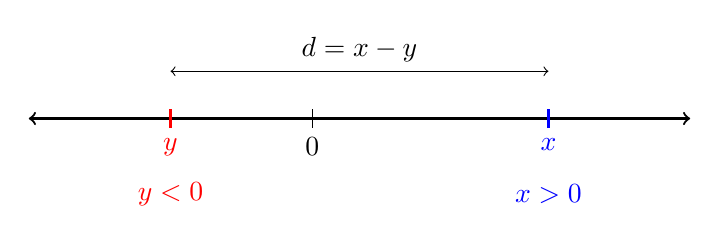
\begin{tikzpicture}[scale=1.2]
    % Number line
    \draw[thick, <->] (-3,0) -- (4,0);
    
    % Tick marks and labels
    \draw (0,0.1) -- (0,-0.1) node[below] {$0$};
    
    % Points on the line
    \draw[red, thick] (-1.5,0.1) -- (-1.5,-0.1) node[below, red] {$y$};
    \draw[blue, thick] (2.5,0.1) -- (2.5,-0.1) node[below, blue] {$x$};

    % Distance indicator showing d = x - y
    \draw[black, <->] (-1.5,0.5) -- (2.5,0.5) node[midway, above] {$d = x - y$};
    
    % Additional labels
    \node[red] at (-1.5, -0.8) {$y < 0$};
    \node[blue] at (2.5, -0.8) {$x > 0$};
    
\end{tikzpicture}
\caption{Number line showing the relationship between $x$, $y$ and $x-y$}
\label{fig:q01_numberline}
\end{figure}

Since $x > 0$ and $y < 0$, we can assume that $x - y = d$ where $d > 0$.

Therefore, $\text{RHS} = |x - y| = d$ is always true.

Now we need to consider cases for $|x + y|$ based on whether $x + y$ is positive or negative.

\vspace{1em}

\textbf{Case I:} $x + y \geq 0$ 

From $x - y = d$, we get $x = y + d$.

Therefore: $x + y = (y + d) + y = 2y + d$

Since $x + y \geq 0$, we have $|x + y| = x + y = 2y + d$.

So $\text{LHS} = 2y + d$ and $\text{RHS} = d$.

Since $y < 0$, we have $2y < 0$, which means $\text{LHS} = 2y + d < d = \text{RHS}$.

\vspace{1em}

\textbf{Case II:} $x + y < 0$

From $x - y = d$, we get $y = x - d$.

Therefore: $x + y = x + (x - d) = 2x - d < 0$

Since $x + y < 0$, we have $|x + y| = -(x + y) = -(2x - d) = d - 2x$.

So $\text{LHS} = d - 2x$ and $\text{RHS} = d$.

Since $x > 0$, we have $2x > 0$, which means $\text{LHS} = d - 2x < d = \text{RHS}$.

\vspace{1em}

\textbf{Conclusion:}

Cases I and II exhaustively cover all possible scenarios. In both cases, we have shown that $\text{LHS} < \text{RHS}$, which means $|x + y| < |x - y|$.

Therefore, we have proven the stronger result: $\boxed{|x + y| \leq |x - y| \text{ for } x > 0, y < 0}$

\textbf{Hence Proved.} $\square$